\documentclass{article} % For LaTeX2e
\usepackage{nips15submit_e,times}
\usepackage{hyperref}
\usepackage{url}
\usepackage{graphicx}
\usepackage{algorithm}  
\usepackage{algorithmic}
\usepackage[colorlinks,linkcolor=blue]{hyperref}
\usepackage{listings}
\usepackage{color}
\usepackage{amssymb}
\usepackage{amsmath}

\definecolor{dkgreen}{rgb}{0,0.6,0}
\definecolor{gray}{rgb}{0.5,0.5,0.5}
\definecolor{mauve}{rgb}{0.58,0,0.82}

\lstset{frame=tb,
  language=Python,
  aboveskip=3mm,
  belowskip=3mm,
  showstringspaces=false,
  columns=flexible,
  basicstyle={\small\ttfamily},
  numbers=none,
  numberstyle=\tiny\color{gray},
  keywordstyle=\color{blue},
  commentstyle=\color{dkgreen},
  stringstyle=\color{mauve},
  breaklines=true,
  breakatwhitespace=true,
  tabsize=3
}

%\documentstyle[nips14submit_09,times,art10]{article} % For LaTeX 2.09


\title{Weekly Report(July 12th, 2019)
}


\author{
David S.~Hippocampus\thanks{ Use footnote for providing further information
about author (webpage, alternative address)---\emph{not} for acknowledging
funding agencies.} \\
Department of Computer Science\\
Cranberry-Lemon University\\
Pittsburgh, PA 15213 \\
\texttt{hippo@cs.cranberry-lemon.edu} \\
\And
Coauthor \\
Jianghao Lin \\
Shanghai Jiao Tong University \\
\texttt{chiangel.ljh@gmail.com} \\
\AND
Coauthor \\
Affiliation \\
Address \\
\texttt{email} \\
\And
Coauthor \\
Affiliation \\
Address \\
\texttt{email} \\
\And
Coauthor \\
Affiliation \\
Address \\
\texttt{email} \\
(if needed)\\
}

% The \author macro works with any number of authors. There are two commands
% used to separate the names and addresses of multiple authors: \And and \AND.
%
% Using \And between authors leaves it to \LaTeX{} to determine where to break
% the lines. Using \AND forces a linebreak at that point. So, if \LaTeX{}
% puts 3 of 4 authors names on the first line, and the last on the second
% line, try using \AND instead of \And before the third author name.

\newcommand{\fix}{\marginpar{FIX}}
\newcommand{\new}{\marginpar{NEW}}

%\nipsfinalcopy % Uncomment for camera-ready version

\begin{document}


\maketitle

\begin{abstract}
This is a collection of my paper notes for future reference.
\end{abstract}

\newpage
\tableofcontents
\newpage

\section{Transposed Convolution}

Transposed Convolution, also known as Deconvolution or Fractionally-strided Convolution, is often used to up-sample images from low resolution to high resolution. Compared with some traditional interpolation method for up-sampling, transposed convolution has learnable parameters.

\newpage

\section{GAN: Generative Adversarial Networks}

\subsection{Basic idea of GAN}

Generative adversarial nets are based on a game theoretic scenario where the generator network directly produces images $x$ from a random noise $z$ and another discriminator network tries to distinguish the generated image from the real ones.

Ideally, the distribution of the generated data will be the same as the real data image and the accuracy of the discriminator network will be $0.5$ because it can not tell an image is actually fake or not.

\subsection{How to measure the divergence ?}

\subsubsection{KL divergence}

KL divergence is also called relative entropy. 

For discrete probability distributions $P$ and $Q$ defined on the same probability space, the KL divergence between $P$ and $Q$ is defined to be:

\begin{equation}
    KL(P||Q) = \sum_{x}P(x)log(\frac{P(x)}{Q(x)})
\end{equation}

For continuous random variables, it is defined to be:

\begin{equation}
    KL(P||Q) = \int_{-\infty}^{\infty}p(x)log(\frac{p(x)}{q(x)})dx
\end{equation}

We can have the inequation because the log function is a convex function: 

\begin{equation}
    \begin{split}
        KL(P||Q) & = \int_{-\infty}^{\infty}p(x)log(\frac{p(x)}{q(x)})dx \\
                 & = -E(log\frac{P(x)}{Q(x)}) \\
                 & \geq -log(E(\frac{P(x)}{Q(x)})) \\
                 & = -log(P(x) \times \frac{P(x)}{Q(x)}) = 0
    \end{split}
\end{equation}

Therefore, KL divergence is in range of $[0, 1]$. KL divergence is equal to $0$ if and only if two distribution is exactly the same. And the smaller the KL divergence is, the more similar two distributions are.

\subsubsection{JS divergence}

It is obvious that KL divergence is asymmetric, which means that $KL(P||Q) \neq KL(Q||P)$. So we introduce the JS divergence:

\begin{equation}
    JS(P||Q) = \frac{1}{2}KL(P||M) + \frac{1}{2}KL(Q||M)
\end{equation}

where $M = \frac{1}{2}(P + Q)$. The range of JS divergence is $[0, log2]$. JS divergence is obviously symmetric and the smaller the JS divergence is, the more similar two distributions are.

\subsection{Definitions in GANs}

\begin{itemize}
    \item \textbf{Generator G} - G is a function that takes a vector $z$ and outputs $x$. So given a prior distribution $P_{z}(z)$, then a probability distribution $P_{G}(x)$ is defined by function G.
    \item \textbf{Discriminator D} - D is a function (actually a binary classification) takes $x$ as inputs and outputs a scalar in range of $[0, 1]$ to tell the input $x$ is faked or not.
    \item \textbf{V(G, D)} - The function V(G, D) is defined to be:
        \begin{equation}
            V(G, D) = E_{x\sim p_{data}}[log(D(x))]+E_{z\sim p_z}[log(1-D(G(z)))]
        \end{equation}
        Defining V(G, D) like this allows the following missions:
            \begin{enumerate}
                \item Given a G, $\max_{D}V(G,D)$ evaluates the difference between $p_G$ and  $p_{data}$.
                \item $\min \limits_{G} \max \limits_{D}V(G, D)$ picks a generator that minimize the difference.
            \end{enumerate}
\end{itemize}

\subsection{Solve $\mathop{\arg\max} \limits_{D}V(G, D)$}

Given a G, thus distribution $p_{G}$ is determined. We have

\begin{equation}
    \begin{split}
        V & = E_{x\sim p_{data}}[log(D(x))]+E_{z\sim p_z}[log(1-D(G(z)))] \\
          & = E_{x\sim p_{data}}[log(D(x))]+E_{x\sim p_G}[log(1-D(x))] \\
          & = \int_{x}p_{data}(x)log(D(x))dx + \int_{x}p_{G}(x)log(1-D(x))dx \\
          & = \int_{x}[p_{data}(x)log(D(x)) + p_{G}(x)log(1-D(x))]dx
    \end{split}
\end{equation}

Because $p_{data}$ and $p_G$ are both fixed, for each input $x$, we can easily compute the result that maximizes $V(G,D)$:

\begin{equation}
    D^{*}(x) = \frac{p_{data}(x)}{p_{data}(x)+p_{G}(x)}
\end{equation}

\subsection{Why $\max \limits_{D} V(G,D)$ evaluates the difference of distributions?}

\begin{equation}
    \begin{split}
        & \quad \max \limits_{D}V(G,D) \\
        & = V(G,D^{*}) \\
        & = E_{x \sim p_{data}}[log\frac{p_{data}(x)}{p_{data}(x)+p_{G}(x)}] + E_{x \sim p_{G}}[log\frac{p_{G}(x)}{p_{data}(x)+p_{G}(x)}] \\
        & = \int_{x}p_{data}(x)log\frac{p_{data}(x) \times \frac{1}{2}}{(p_{data}(x)+p_{G}(x)) \times \frac{1}{2}}dx \\
        & \quad \ \  + \int_{x}p_{G}(x)log\frac{p_{G}(x)}{\frac{1}{2}(p_{data}(x)+p_{G}(x)) \times \frac{1}{2}}dx \\
        & = -2log2 + \int_{x}p_{data}(x)log\frac{p_{data}(x)}{\frac{1}{2}(p_{data}(x)+p_{G}(x))}dx \\
        & \quad \ \  + \int_{x}p_{G}(x)log\frac{p_{G}(x)}{\frac{1}{2}(p_{data}(x)+p_{G}(x))}dx \\
        & = -2log2 + KL(p_{data}||\frac{p_{data}+p_G}{2} + KL(p_{G}||\frac{p_{data}+p_G}{2}) \\
        & = -2log2 + JS(p_{data}||p_G)
    \end{split}
\end{equation}

Therefore, we can see that $V(G,D^{*})$ is the sum of a JS divergence and a constant $-2log2$. So it can evaluate the difference of distributions. And the smaller the $V(G,D^{*})$ is, the more similar $p_{data}$ and $p_G$ are.

\subsection{Final target - the generator}

Our final aim is to achieve a generator G that have the same distribution $p_G$ as $p_{data}$, which means the smallest divergence. So our optimal objective is

\begin{equation}
    G^{*} = \arg \min \limits_{G} \max \limits_{D} V(G,D)
\end{equation}

\subsection{Tips for implementing a GAN}

\begin{enumerate}
    \item Due to the difficulty of computing the real expectation of distributions, we use the arithmetic mean of samples $\{x^(1),...,x^{(m)}\}$ and $\{z^{(1)},...,z^{(m)}\}$ to approximate it:
        \begin{equation}
            \frac{1}{m}\sum_{i=1}^{m}[log(D(x^{(i)}))+log(1-D(G(z^{(i)})))]
        \end{equation}
    \item Update the generator by descending the following stochastic gradient can be inefficient:
        \begin{equation}
            \nabla_{\theta_{G}}\frac{1}{m}\sum_{i=1}^{m}log(1-D(G(z^{(i)})))
        \end{equation}
    Because the equation indicates that the more real the generated image $z$ is, the smaller the gradient is. That is, the gradient will be almost $0$ at the begin of training and increase significantly when the generator is able to generate a good enough image! This will make the training inefficient and uneasy to converge.
    So we usually use the gradient below as an alternative. More real the image, less the gradient.
        \begin{equation}
            \nabla_{\theta_{G}}\frac{1}{m}\sum_{i=1}^{m}log(D(G(z^{(i)})))
        \end{equation}
\end{enumerate}

\newpage

\section{DCGAN: Deep Convolutional Generative Adversarial Network}

\subsection{Architecture guidelines for stable DCGANs}

\begin{enumerate}
    \item Do not use any pooling layers. Use strided convolutional layers in discriminator network and fractional-strided convolutional layers in generator network instead.
    \item Use batch normalization in both generator and discriminator network. Note that directly applying batch normalization to all layers may result in sample oscillation and instability. In order to avoid this situation, do not apply batch normalization to the output layer of generator and the input layer of discriminator.
    \item Do not use any fully connected layers. We can use global pooling instead which contributes to model stability but slow down the convergence.
    \item Use ReLU activation in generator network for all layers except for the output layer which uses tanh activation to project values to $[-1, 1]$.
    \item Use Leaky ReLU in all layers of discriminator network.
\end{enumerate}

\subsection{Training details for DCGANs}

\begin{enumerate}
    \item No pre-processing. Only use tanh activation to scale the range of value into $[-1,1]$
    \item SGD
    \item Batch size of $128$
    \item All weights are initialized from a zero-center normal distribution with standard deviation $0.02$
    \item The slope of Leaky ReLU is $0.2$
    \item Adam optimizer
    \item Learning rate of $0.0002$
    \item Momentum term $\beta_1$ is $0.5$ instead of $0.9$
\end{enumerate}

\subsection{Validate the model capacity}

In this part, the author mainly measure the capacity of discriminator network as feature extractors compared with other unsupervised learning methods.

\subsubsection{CIFAR dataset}

We use all convolutional layers of discriminator which comes from a pre-trained DCGAN model on Imagenet-1k. We maxpool each layer representation to produce a $4 \times 4$ spatial grid. We then flatten and concatenate these grids to form a $28672$ dimensional vector. By putting the output of the feature vector into a L2-SVM linear model, we can get a classification scores for supervised learning tasks.

As a result, DCGAN+L2-SVM performs better than k-means baseline method but is not as good as the Exemplar CNN(another method to apply unsupervised learning tasks with CNN).

\subsubsection{SVHN dataset}

After the similar approach above, we can transfer the discriminator' convolutional layers into feature vector and put it with L2-SVM. This time, DCGAN+L2-SVM outperform the previous works when labeled data is scarce.

\subsection{Visualization}

In this part, the author wants to mainly validate that the DCGAN model is actually learning features and representation from the image instead of simply memorizing and fitting the input image. The demonstration is various and imaginative.

\subsubsection{Walking in the latent space}

Interpolation applied to latent vector $z$ results in smooth transition on the generated images. E.g. images transfer from having windows to not having windows. This indicates the feature representation in latent vector $z$.

\subsubsection{Visualizing discriminator features}

Using the \emph{guided backpropagation}, we can visualize the last convolutional layer of discriminator network. And we can see many base outline of specific objects like a mirror or a window. This indicates the features learned in discriminator network.

\subsubsection{Visualizing generator features}

The author do the following two experiments, which strongly demonstrate that there is feature hierarchy architecture in generator network.

\begin{enumerate}
    \item \textbf{Eliminate objects by modifying the generator} - Use logistic regression to predict whether a feature activation is on a window or not based on $150$ manually labeled generated images. Drop all activations that are greater than zero(indicating a window). Then, applying the same vector $z$, generator network will produce image without window accordingly! But the generated image is also blurrier.
    \item \textbf{Vector arithmetic} - Applying vector arithmetic on input $z$ will result in feature object combination or elimination.
\end{enumerate}

\newpage

\section{CGAN: Conditional Generative Adversarial Network}

\subsection{Motivations}

In the previous GAN models, we can not control the kind of images we will generate from a random noise $z$. That is, from a random noise $z$, we may generate a cat image, a dog image and so on. It is kind of out of control.

But in CGAN, by adding additional information like class labels or textual descriptions, we can somehow control the type of the generated images. 

The general architecture of CGAN are shown in figure \ref{fig:CGAN}.

\begin{figure}[h]
	\centering
	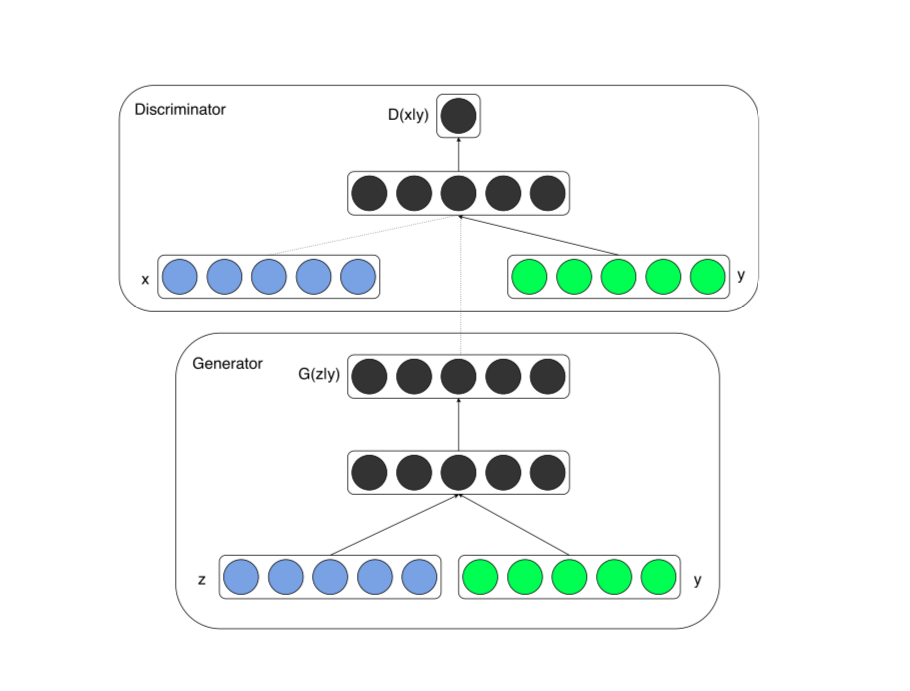
\includegraphics[width=0.9\linewidth]{figures/CGAN.png}
	\caption{Architecture of CGAN}
	\label{fig:CGAN}
\end{figure}

\subsection{How to combine the inputs ?}

It is not hard to get the core idea of CGAN. But what really confused me a while is how do we actually combine those inputs $z$ and $y$ together and feed it to the network?

As we are trying to model the joint conditional, the simplest way to do it is to just concatenate both variables. Hence, in $G(z,y)$, we are concatenating $z$ and $y$ before we feed it into the networks. The same procedure is applied to $D(X,y)$. Also we can apply other data process to $y$ before we concatenate it with $z$ like a fully connected layer if needed.

\section{}

\end{document}